% KERdoc.tex V1.0, 14 June 2004

\documentclass{kerauth}
\usepackage{graphicx}
\usepackage{pdfpages}
%\usepackage{times}

\usepackage{natbib}
\usepackage[hidelinks]{hyperref}
\bibliographystyle{humannat}
%\setcitestyle{authoryear,open={(},close={)}}

\begin{document}
\KER{1}{24}{00}{0}{2004}{S000000000000000}

\KER{0}{0}{00}{0}{2015}{S000000000000000}
\runningheads{Nguyen et al.}{Knowledge engineering on PhD stories: bottom-up vs. goal-directed approach}
%\doublespacing
\title{Knowledge engineering on PhD stories: bottom-up vs. goal-directed approach}
\author{VIET BACH NGUYEN\affilnum{1},
STANISLAV KRUML\affilnum{1}, 
VOJT\v{E}CH SV\'{A}TEK\affilnum{1} and 
ÓSCAR CORCHO\affilnum{2}}
\address{\affilnum{1}Prague University of Economics and Business, N\'{a}m. W. Churchilla 4, 130 67 Praha 3, Czech Republic\\
\email{viet.nguyen@vse.cz  krus02@vse.cz svatek@vse.cz}\\
\affilnum{2}Universidad Politécnica de Madrid, Madrid, Spain\\
\email{ocorcho@fi.upm.es}
}

\begin{abstract}
Stories of concrete PhD students, reflected in various information sources, are potentially a useful source of reflections and analytics on the underlying generic processes and regulations, and can subsequently give rise to guidelines and hints making the life of future PhD students easier.
The collected information on PhD stories is of quite heterogeneous nature, from structured `master data' from study information systems, through various partial records in broader (e.g., publication) databases, to textually expressed  chronologies, impressions, and lessons learned prepared by the PhD students themselves.
We explored two fundamentally different approaches to arrive at a structured representation of individual PhD stories.
The first approach is bottom-up, relying on aspect-based sentiment analysis (SA) as an established NLP method. 
Training data was collected in the form of 35 textual stories (or, more broadly, documents reflecting the PhD experience of the author), manually labeled by volunteers, and submitted to state-of-the-art SA tools.
The second approach is primarily manual in its nature, though amenable to knowledge/database support: population of a knowledge graph (or, concept map) from primarily structured sources as well as insider information, guided by a hierarchical system of (PhD study) goals. 
The task was accomplished, as a mere proof of concept, by two senior academics with ample experience in supervising PhD students.
Both approaches appear complementary, but insufficient overall, to date. 
While the bottom-up one can much better scale, the result is largely incomplete in its coverage. 
The goal-directed approach is, in turn, extremely demanding on human expertise and laborious due to lack of proper tooling.
Based on the gained experience, we discuss conditions that could allow making knowledge engineering on PhD stories more efficient and effective in the future.

%Support for PhD students and their advisors in decision-making before and along their PhD journeys requires providing them with a deep understanding and knowledge of the life-cycle of a PhD.
%This means giving them access to a thorough understanding of causal relations between events, decisions, and the possible outcome, depending on various states of the PhD student as well as previous experience. 
%This knowledge can be attained primarily from insider documented stories, study reports, communications threads with advisors and colleagues, interviews, and scholarly databases.
%However, it is unclear how to give this knowledge a reasonable structure (due to the heterogeneity of concepts and data sources) so that we can use it for decision-making during the PhD journey.
%In this paper, we explore how to analyze and model PhD stories to uncover, extract causal relationships found within each story to get insights into the co-occurrences and causalities. Specifically, analyze these stories with thematic analysis to understand their main points and we use concept maps to create semi-formal graphs of connected events and objects where the relationships are being emphasized from the perspective of cause and effect. 
%Our results at this point are a collection of PhD stories in the form of concept maps, thematic codes, a proposed approach for goal-directed PhD story modeling described in this paper.
\end{abstract}

\section{Introduction}

The research follows up with an initial pilot \cite{NguyenKCAP21}, which however only featured the clean bottom-up approach in the form of thematic codes being provisionally assigned to twelve documents by a single researcher, and several ad hoc variants of graph modeling, without the support of any explicit guidelines.
The current research, in contrast, newly introduces aspect-based sentiment analysis as a particular computational technique, in the bottom-up approach, and standardizes the graph modeling (goal-driven) approach through common guidelines.
The total size of the collection has doubled (tripled).
Explicit formulation of requirements allowing for effective knowledge engineering in the given domain is yet another contribution of the paper.

The structure of this paper is as follows: 

\section{Related research}
\label{s:related}

\subsection{PhD story analysis}
\subsection{Academic knowledge graphs}
\subsection{Biography modeling}

\section{Bottom-up analysis}
\label{s:data-bottom}
\subsection{Data collection}
The PhD story data used in this research are mostly acquired from websites where they are published by their respective authors or by the permitted publishers. Apart from that, we also have gathered several ``offline'' stories via face-to-face interviews. Fig. \ref{fig:data-collection} briefly shows our web search strategy along with the proportion of the resources by each document type.

\begin{figure}[ht]
  \centering
  % drawio file: https://app.diagrams.net/#G1uuesc5QGArXj6BOuYHoi2sxlLcHhHyJq
  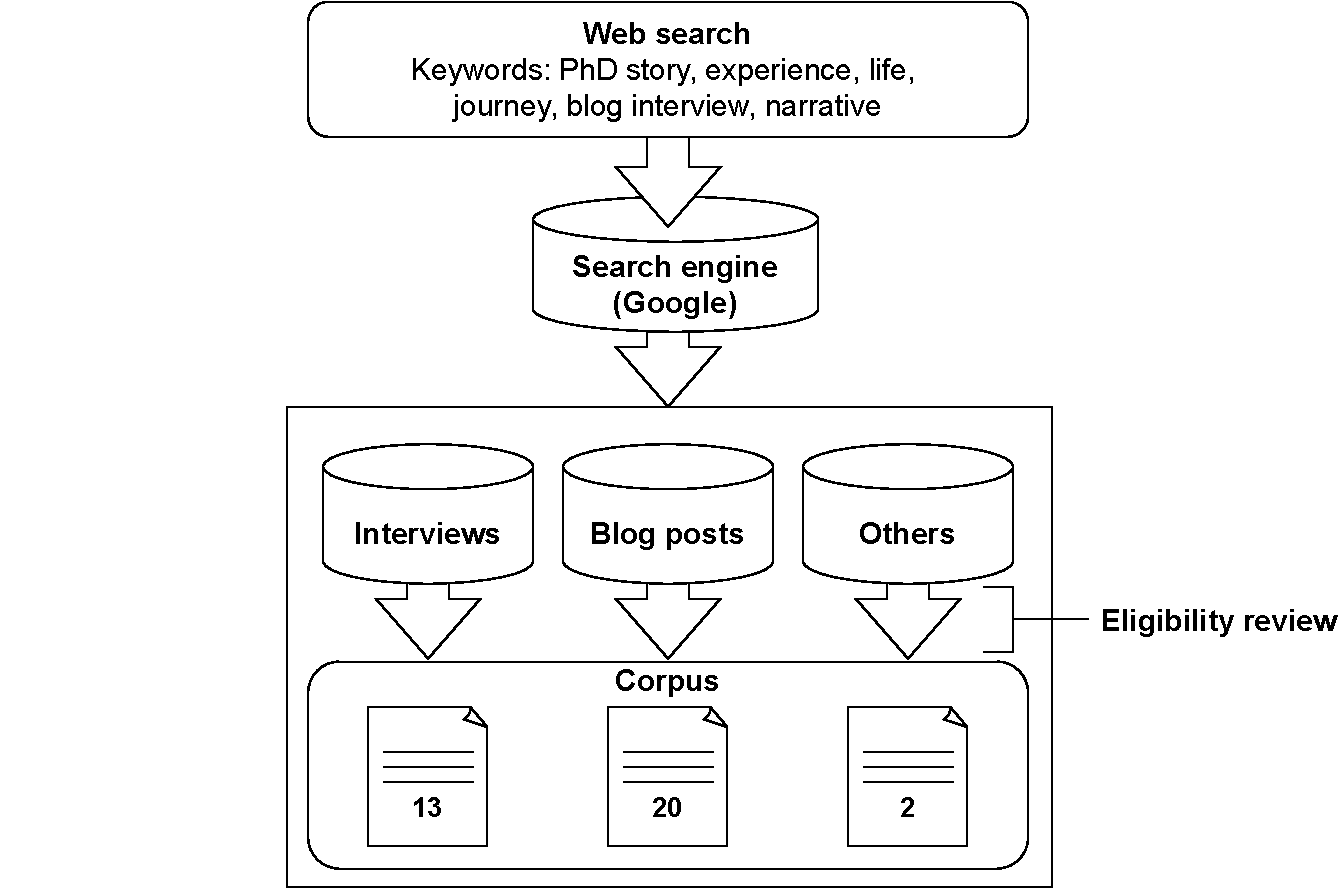
\includegraphics[width=13cm]{figures/data-collection.drawio.pdf}
  \caption[data-collection]{Data collection strategy}% for PhD story analysis and modeling}
  \label{fig:data-collection}
\end{figure}

To collect stories that are published online, we follow a simple keyword-based search strategy on Google to produce results in the form of links. In this search strategy, suitable keywords are defined to search for PhD stories. These keywords are \textit{PhD story}, \textit{my PhD story}, \textit{my PhD journey}, \textit{PhD narrative}, \textit{PhD experience}, \textit{PhD blog}, \textit{PhD interview}, \textit{PhD life}, and some combinations. Next, we visit each link and quickly scan the story content to determine whether a story is eligible for further analysis. Our selection criteria are not strictly defined, since every story is unique in writing style, form, and thoughts being conveyed. However, the most important first-hand properties we look for in the stories during the web search are language (only English), summarizing intent, sufficient story length (e.g., approximately five hundred words or more), high coverage of multiple PhD life aspects\footnote{...list the aspects from the aspect analysis phase}, high density in retrospective narrations (e.g., lesson learned, experience, situations, decisions), chronological composition (e.g., sectioned into academic years), and recentness of the story (e.g., we only consider modern PhD experiences, thus only stories published in the last 20 years are collected, this should exclude PhD programs active in the 1990s and earlier).

In other words, the search results are filtered\footnote{We do not filter the stories based on the research field of the authors, but we initially wanted to limit our search scope to Applied Informatics only. We decided to drop this criterion since the initial number of search results was not enough. We then expanded our search scope to the Computer Science domain, but again the search yielded too few results. Therefore, after removing this limitation, our final dataset contains stories from different research domains, such as biology, physics, maths, engineering, literature, etc.}, and if the data do not satisfy the above-mentioned criteria, they are omitted. In the case of ``offline'' interviews, we guided the interviewees with our open interview questions to allow them to speak freely but also to gather the needed information. These interview records were later transcribed into text and included in the final dataset. Our dataset is a corpus of a total of 35 eligible PhD stories in textual form with about a total of 76\,088 words, ranging from 500 words to 6\,000 words each and the average word count is 2\,174. We classify the document types into blog posts (20), interviews (13), and others (1 vlog and 1 web article).


\subsection{Document categorization}
Since the nature of the documents varied, we manually skimmed them so as to establish categories (clusters) of documents having similar natures and/or destinations.
...
\subsection{Aspect system design}
We design the aspects via brainstorming where we list out different areas and topics that a PhD student may talk about. Also, with the consultancy of our senior member, we have created the following tree of aspects to be used during aspect annotation


\begin{figure}[ht]
  \centering
  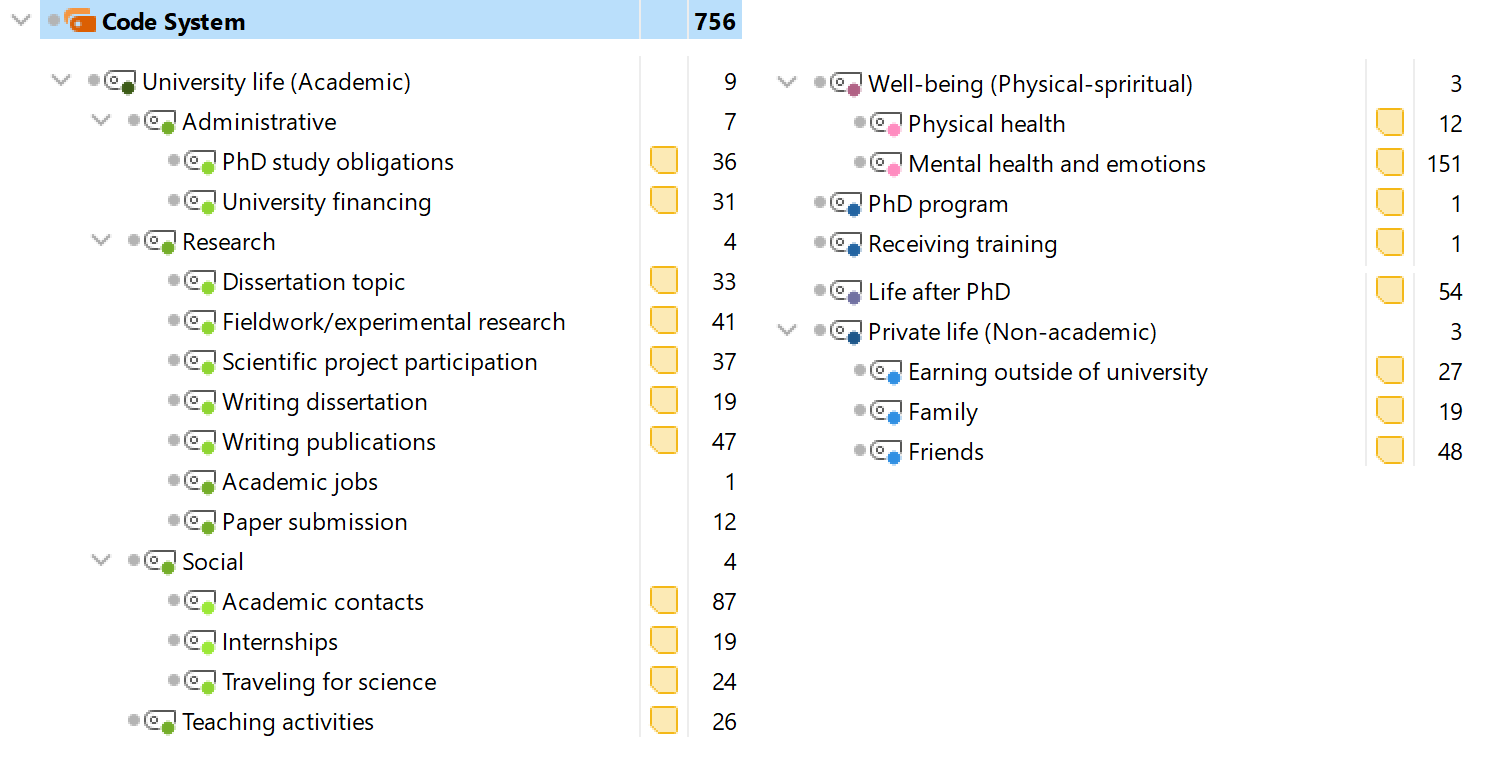
\includegraphics[width=15cm]{figures/aspect-codes.png}
  \caption[aspect-codes]{Annotation codes -- aspects}
  \label{fig:aspect-codes}
\end{figure}

\subsection{Aspect annotation}
We annotate the collection of PhD stories using MAXQDA software. For this annotation of aspects, we had a team of 6 people annotating 24 stories (at the time we only had 24 stories), see Tab. \ref{aspect-annotation-pools}. Each person took care of 6 stories so that 12 stories are annotated once and the 12 stories are annotated twice by two people in hopes of measuring the annotators' agreement. We split the 24 stories into 6 pools evenly so that the time spent in each story pool would be approximately the same as in other pools. The time measured is based on the total word count of the stories in each pool. We approximated the reading and annotating speed to 100 words per minute while the average reading speed of an adult person is around 238 words per minute. The reported time spent in each pool by the annotators turned out to be approximately the same. In this aspect annotation phase, we have produced a total of 756 annotations.

\begin{table}[ht]
\small
\centering
\begin{tabular}{|c|l|c|c|l|}
\hline
% data: https://docs.google.com/spreadsheets/d/1xljwRX6YQHD_14wqtuRoIbZwUhkDr4QI
\textbf{pool} & \textbf{files to annotate} & \textbf{time estimate {[}m{]}} & \textbf{word count} & \textbf{annotator} \\ \hline
A             & 09, 13, 17, 18, 20, 21     & 119                            & 12\,182               & Vojta              \\ \hline
B             & 02, 06, 08, 13, 14, 19     & 114                            & 11\,630               & Standa             \\ \hline
C             & 01, 03, 06, 08, 11, 15     & 120                            & 12\,245               & David              \\ \hline
D             & 01, 04, 05, 10, 12, 23     & 110                            & 11\,083               & Marek              \\ \hline
E             & 03, 16, 17, 19, 22, 23     & 123                            & 12\,515               & Bach               \\ \hline
F             & 07, 10, 12, 15, 21, 24     & 122                            & 12\,419               & Gollam             \\ \hline
\end{tabular}
\caption[aspect-annotation-pools]{Aspect annotation pools}
\label{aspect-annotation-pools}
\end{table}+

\subsection{Polarity and emotion annotation}
Aside from three-valued polarity, we also used this opportunity to acquire information on the \emph{surprise} emotion.
The reason is that the surprise emotion is one that does not inherently lean towards positive nor negative polarity, yet can be an important ingredient in a PhD student's story -- whether in the context of the actual research (succeeding or failing against odds) or, e.g., social relationships within the lab or school.


\begin{figure}[ht]
  \centering
  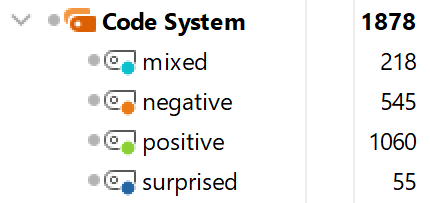
\includegraphics[width=5cm]{figures/sentiment-codes.png}
  \caption[sentiment-codes]{Annotation codes -- sentiments}
  \label{fig:sentiment-codes}
\end{figure}

We also annotate our collection of PhD stories with sentiments using MAXQDA software. This time we had a different team of 8 people manually annotate all 35 stories using 4 annotation codes which are \textit{positive}, \textit{neutral}, \textit{negative}, and the mentioned \textit{surprise} emotion. For this annotation task, we divide our corpus of stories into 8 distinct pools with 6--7 stories each so that 18 stories are annotated twice by two people. Each pool represents about 155 minutes of reading and annotating time for approximately 15\,500 words (we stick with the speed of 100 words per minute from the aspect annotation phase). We calculate these estimated time values based on the word count of each document and distribute the stories into the pool evenly by time, see Tab. \ref{sentiment-annotation-pools}. 

\begin{table}[ht]
\small
\centering
\begin{tabular}{|c|l|c|c|l|}
\hline
% data: https://docs.google.com/spreadsheets/d/1cuud9l3o3q_SlVWcSTW2Vidgn25DRC3M
\textbf{pool} & \textbf{files to annotate}    & \textbf{time estimate {[}m{]}} & \textbf{total words} & \textbf{annotator} \\ \hline
A             & 17, 20, 22, 25, 29, 31, 32    & 151                            & 15\,105              & Dominik            \\ \hline
B             & 08, 13, 14, 15, 28, 34, 35    & 146                            & 14\,642              & Šimon              \\ \hline
C             & 06, 08, 10, 19, 27, 30        & 160                            & 16\,045              & Michael            \\ \hline
D             & 01, 02, 04, 05, 23, 25, 27    & 161                            & 16\,080              & Dominika           \\ \hline
E             & 01, 03, 13, 17, 21, 23, 26    & 149                            & 14\,863              & Karel              \\ \hline
F             & 07, 10, 12, 15, 24, 33, 35    & 151                            & 15\,069              & Maxim              \\ \hline
G             & 03, 06, 09, 18, 19, 29        & 151                            & 15\,148              & Kateřina           \\ \hline
H             & 11, 12, 16, 21, 31, 33        & 159                            & 15\,876              & Marek              \\ \hline
\end{tabular}
\caption[sentiment-annotation-pools]{Sentiment annotation pools}
\label{sentiment-annotation-pools}
\end{table}

Annotators were then randomly assigned to these pools. We also provide the annotators with a common guide document explaining the necessary steps for the annotations. Our definitions of sentiment values are the following:

\begin{itemize}
    \item \textit{positive} -- there is an explicit or implicit clue in the sentence suggesting the writer’s attitude towards or judgment of the subject is positive (thankful, excited, optimistic, overjoyed, happy, inspired, etc.),
    \item \textit{negative} -- there is an explicit or implicit clue in the sentence suggesting the writer's attitude towards or judgment of the subject is negative (critical, angry, disappointed, pessimistic, sarcastic, mocking, bored, complaint, etc.),
    \item \textit{mixed} -- there is an explicit or implicit clue in the sentence suggesting that the writer's attitude towards or judgment of the subject is both positive and negative,
    \item \textit{unknown} -- there is no explicit or implicit clue indicating that the writer feels positively or negatively about the subject (this value is not used during the annotation process, whatever text that remains after annotating is considered unknown)
\end{itemize}

Each annotated sentence can only have 1 sentiment (positive, mixed, or negative -- these are disjoint). However, these sentences may also include a surprise emotion, such as when there is a sentence containing ''I didn’t know``, or ''it was nothing like I imagined``, etc. In that case, they should also be annotated with the \textit{surprised} emotion code. In this sentiment annotation phase, a total of 1878 annotations are created.

\subsection{Sentiment analysis: employed techniques}
\subsection{Sentiment analysis: results}

\section{Goal-directed analysis}
\label{s:goal}

\subsection{Data sources}
\label{s:data-goal}

\subsection{Modeling guidelines}
\label{s:guid}

\subsection{Produced concept graphs}
\label{s:graps}

accessibility of Semantic Scholar in ContextMinds

\section{Discussion}

\section{Conclusion}
\label{s:concl}

Future: fetching data from DBLP and similar databases

\acks
This research was supported by VSE IGS F4/56/2021.
The authors are indebted to the volunteer annotators, without whom the research described in Section~\ref{s:data-bottom} would not have been possible. % include names for those who agree?

\bibliography{references}
\end{document}